\section{Алгоритм \quotes{Bundle adjustment}}

\textbf{Bundle adjustment} (дословно \quotes{\textit{регулировка пучков}}) - алгоритм проективной геометрии который, решая системы нелинейных уравнений (путем минимизации ошибки) находит 3d координаты ключевых точек в пространстве. Используется на последних этапах процесса Structure from Motion.

Одна трёхмерная точка в реконструируемой модели соответствует нескольким двухмерным точкам на исходных изображениях (потому что на снимках изображено одна и та же местность или объект с разных ракурсов). Если спроецировать 3d точку на изображения - лучи должны попасть в соответствующие ей 2d точки. И, в свою очередь, все лучи должны собраться в один \quotes{пучок} в точке на трёхмерной модели.

Суть метода Bundle adjustment:
\begin{enumerate}
    \item Представление всех лучей, которые должны сойтись в одной точке как систему алгебраических уравнений;
    \item Нахождение ошибки между проекцией и реальной точкой на изображении;
    \item Минимизация этой ошибки путем решения систем нелинейных уравнений и передвижения камер (изображений);
    \item В конечном итоге получение такого расположения исходных изображений в 3d пространстве, что лучи соответствующие одной точке собираются в один пучок с минимально возможной ошибкой.
\end{enumerate}

\begin{figure}[h]
    \centering
    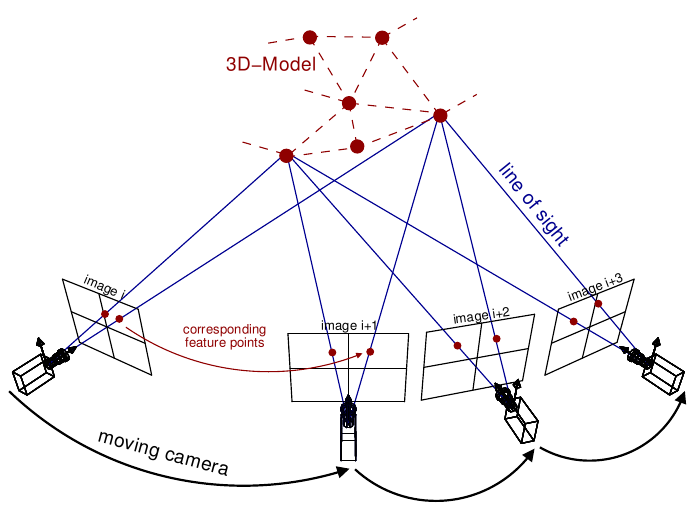
\includegraphics[width=1\textwidth]{images/bundle_adjustment.png}
    \caption{\textbf{Пример работы Bundle adjustment}}
    \label{fig:ba}
\end{figure}

На рисунке \ref{fig:ba} проиллюстрировано, как в процессе работы алгоритма меняется расположения исходных камер для нахождения истинных координат трёхмерной точки.
